% Adapted from the author's public Erdos Paper IV v1.23 series_template.tex.
% Layout provenance is recorded in 02_validation; the Markdown is semantic authority.
\documentclass[english,11pt,a4paper]{article}
\usepackage[margin=1in]{geometry}
\usepackage{fontspec}
\setmainfont{lmroman10-regular.otf}[BoldFont=lmroman10-bold.otf,ItalicFont=lmroman10-italic.otf,BoldItalicFont=lmroman10-bolditalic.otf]
\setsansfont{lmsans10-regular.otf}[BoldFont=lmsans10-bold.otf]
\setmonofont{lmmono10-regular.otf}[Scale=MatchLowercase]
\usepackage{amsmath,amssymb}
\providecommand{\mathscr}{\mathcal}
\usepackage[english]{babel}
\usepackage{microtype,parskip}
\usepackage{longtable,booktabs,array,calc}
\usepackage{xcolor,xurl}
\usepackage{hyperref,bookmark}
\usepackage{etoolbox,needspace}
\setcounter{secnumdepth}{-\maxdimen}
\setlength{\emergencystretch}{3em}
\providecommand{\tightlist}{\setlength{\itemsep}{0pt}\setlength{\parskip}{0pt}}
\newcounter{none}
\AtBeginEnvironment{longtable}{\Needspace{8\baselineskip}\small}
\pretocmd{\section}{\Needspace{5\baselineskip}}{}{}
\pretocmd{\subsection}{\Needspace{7\baselineskip}}{}{}
\pretocmd{\subsubsection}{\Needspace{6\baselineskip}}{}{}
\urlstyle{same}

\usepackage{graphicx}
\providecommand{\pandocbounded}[1]{#1}

\usepackage{float}

\clubpenalty=10000\widowpenalty=10000\displaywidowpenalty=10000
\usepackage{tikz}
\AtBeginEnvironment{longtable}{\Needspace{16\baselineskip}}
\hypersetup{pdftitle={Counting Steiner designs with prescribed color profiles},pdfauthor={Juan Pablo Traverso Gianini},pdflang={en},colorlinks=true,linkcolor=blue,urlcolor=blue,citecolor=blue}
\title{Counting Steiner designs with prescribed color profiles}
\author{Juan Pablo Traverso Gianini\\\small Independent researcher, Santiago, Chile\\\small \href{mailto:jtraverso@gmail.com}{jtraverso@gmail.com}\\\small \href{https://orcid.org/0009-0003-6068-4096}{ORCID: 0009-0003-6068-4096}}\date{}\begin{document}\raggedbottom\maketitle
\begin{center}
\textbf{Paper III. Combinatorial entropy and counting.}\\
\textbf{Preprint 1.0 --- November 24, 2026.}\\
DOI: \url{https://doi.org/10.5281/zenodo.24501236}.\\
\href{https://github.com/jtraverso/latinon-entropy-ldp/tree/main/preprints/STEINER-PROFILES/05_formalization/lean}{Lean sources in the series repository}\end{center}
\subsection{Abstract}\label{abstract}

Given a partition of a labeled \(n\)-element set into \(k\) color classes of linear size, we count the Steiner designs \(S(2,q,n)\) with exactly \(m_\tau\) blocks of each color multiset \(\tau\). For fixed \(q\ge3\) and \(k\), the estimate is uniform over integer quotas satisfying the pair margins and ordinary divisibility conditions, provided every type accounts for a fixed positive fraction of the blocks. Relative to the unrestricted count, the logarithmic cost is \(bD(Q\|P)\), where \(b\) is the number of blocks, \(Q\) is the prescribed type law and \(P\) is the type law of a uniform \(q\)-subset. Both bounds have a power saving in the error. The lower bound uses a weighted random packing and a family of trades that corrects the integer quotas after the uncovered pairs have been absorbed. The enumeration also gives a large-deviation principle on the feasible polytope. At a boundary profile, the lower bound applies to each open neighborhood through approximation by interior profiles.

MSC 2020: 05B05, 05A16, 60F10. Keywords: Steiner designs; color profiles; enumeration; relative entropy; large deviations.

\begin{center}\rule{0.5\linewidth}{0.5pt}\end{center}

\subsection{1. Introduction}\label{introduction}

\subsubsection{1.1 Background}\label{background}

Suppose the points of a Steiner design are colored red and blue. A block with \(j\) red points uses \(\binom j2\) red pairs and \(j(q-j)\) mixed pairs. Since every pair occurs once, prescribing more blocks of one type forces changes in the others. The pair counts tell us which linear equations these changes must satisfy. The enumeration problem asks how many designs realize a particular integer solution.

Paper I of this series counted Latin squares near a prescribed Latinon {[}6{]}. Paper II passed from neighborhoods to exact color statistics. In particular, its Theorem 1.5 counted Steiner triple systems with a prescribed interior profile, and its Corollary 1.6 gave the resulting profile large deviations {[}2{]}. Here the blocks can have any fixed size \(q\ge3\). The extension requires a supply of trades for every integral change of profile that preserves pair counts. Section 3 constructs them on the same vertex set as the packing.

\subsubsection{1.2 The enumeration theorem}\label{the-enumeration-theorem}

Fix a coloring of \([n]\) with \(k\) colors and write \(n_i\) for the size of class \(i\). A block of a Steiner design \(S(2,q,n)\) is a \(q\)-set, and each pair of points belongs to exactly one block. Its type \(\tau=(\tau_i)\) records the number of points of each color. Put \(r=\binom q2\). The number of blocks in a design and the number of possible blocks of type \(\tau\) are respectively \[b=\frac{\binom n2}{r},\qquad N_\tau=\prod_i\binom{n_i}{\tau_i}.\] Each column of the matrix \(A_{u,\tau}=\prod_i\binom{\tau_i}{u_i}\) counts the pairs in one block, grouped by their color multiset \(u\). Thus an integer histogram \(m\) must satisfy \((Am)_u=\prod_i\binom{n_i}{u_i}\) for every pair type \(u\). Summing these equations gives \(\sum_\tau m_\tau=b\). For the fixed coloring \(\chi\), write \(N(m)=N_\chi(m)\) for the number of designs on this labeled point set with histogram \(m\).

A uniform block of a design in this fiber has type law \(Q_\tau=m_\tau/b\). A uniform \(q\)-set of points has type law \(P_\tau=N_\tau/\binom nq\). Write \(D(Q\|P)=\sum_\tau Q_\tau\log(Q_\tau/P_\tau)\), with zero contribution from a type of zero mass. Each pair lies in \(d_0=\binom{n-2}{q-2}\) possible blocks. Our estimate is centered at \[\Phi(m)=b\,[\log d_0-(r-1)-D(Q\|P)]. \tag{1}\]

\Needspace{7\baselineskip}\textbf{Theorem 1.1.} Fix \(q\ge3\), \(k\ge1\) and \(\rho,\kappa>0\). There are constants \(C,n_0\) such that the following holds for all \(n\ge n_0\). Suppose \(r\mid\binom n2\), \(q-1\mid n-1\), and every color class has size at least \(\rho n\). For every integer histogram \(m\) satisfying the pair margins and \(m_\tau\ge\kappa b\) for all \(\tau\), there is a design in the fiber, and \[\Phi(m)-C n^{2-z}\log n\ \le\ \log N(m)\
 \le\ \Phi(m)+C n^{2-1/(r-1)},\qquad
 z=\frac{1}{(4r-1)(2q-1)+2}. \tag{2}\] The upper bound in multiplicative form, \(N(m)\le\exp(\Phi(m)+C n^{2-1/(r-1)})\), holds for all nonnegative integer quotas with these margins. In particular it applies to empty fibers. The lower bound is uniform on each fixed interior region. In Section 10 we approximate a boundary point by interior profiles to obtain a probability bound for every open neighborhood of that point.

Closed events in Section 10 can include types of zero mass, so we will use the upper estimate precisely there. For block sizes \(3,4,5\), the lower-bound exponent \(z\) is \(1/57,1/163,1/353\), respectively. These are asymptotic savings for fixed \(q\).

\subsubsection{1.3 Relation to earlier work and outline of the proof}\label{relation-to-earlier-work-and-outline-of-the-proof}

With a single color, the main term is the logarithm of Keevash's unrestricted design count {[}1, Theorem 6.1{]}. His treatment extends the entropy argument of Linial and Luria for triple systems {[}4{]} to general designs. Keevash's work on colored and directed designs places decomposition problems with prescribed edge colors and partite structure in a common existence framework {[}7, 8{]}. Kwan, Sah and Sawhney give upper estimates for the number of clique decompositions with specified numbers of cliques of each size {[}9, §2.2{]}. Here every clique has the same size. Its type depends on the colors of its vertices, and we specify the exact number of cliques of each such type.

For the lower bound, we assign each potential block of type \(\tau\) the weight \(m_\tau/N_\tau\). The pair margins make each pair carry total weight one. Random greedy matching is a classical way of turning nearly uniform loads into an almost complete packing {[}1, 10{]}. In our setting the weights also prescribe frequencies, and even a small error in a frequency matters at the last step. We therefore set aside three edge sets before starting. Table 1 distinguishes their roles. Lemma 3.1 shows why the reserved trades suffice: their histogram differences generate every integral change allowed by the pair margins. Sections 2--5 control the packing, Sections 6--7 complete it with the exact histogram, and Section 8 counts the choices that lead to distinct designs. Section 9 gives the entropy upper bound.

{\def\LTcaptype{none} % do not increment counter
\begin{longtable}[]{@{}
  >{\raggedright\arraybackslash}p{(\linewidth - 4\tabcolsep) * \real{0.3333}}
  >{\raggedright\arraybackslash}p{(\linewidth - 4\tabcolsep) * \real{0.3333}}
  >{\raggedright\arraybackslash}p{(\linewidth - 4\tabcolsep) * \real{0.3333}}@{}}
\toprule\noalign{}
\begin{minipage}[b]{\linewidth}\raggedright
Edges set aside
\end{minipage} & \begin{minipage}[b]{\linewidth}\raggedright
Choice available at completion
\end{minipage} & \begin{minipage}[b]{\linewidth}\raggedright
Quantity controlled
\end{minipage} \\
\midrule\noalign{}
\endhead
\bottomrule\noalign{}
\endlastfoot
Reserve & Extend uncovered edges to cliques using spare pairs & Maximum degree of the uncovered graph \\
Omniabsorber & Decompose it together with the divisible part of the reserve still unused & Coverage of every pair \\
Trade cells & Switch between two decompositions of the same edges & Exact integer histogram \\
\end{longtable}
}

Table 1. Roles of the three edge sets reserved before the random greedy packing.

\subsection{2. Repairing the weights after edge deletions}\label{repairing-the-weights-after-edge-deletions}

Write \(\lambda_B=m_\tau/N_\tau\) for a block \(B\) of type \(\tau\). The total load on pairs of type \(u\) is \((Am)_u\). Permutations within color classes act transitively on these pairs, so they all carry the same load, namely one. The interior hypotheses also put every \(\lambda_B\) between two positive constant multiples of \(n^{2-q}\).

Removing the edges needed at completion removes all blocks containing them. Let \(J\) be the remaining graph and let \(H_J\) be its edge-by-clique incidence matrix. To correct an edge-load error \(h\) we need a right inverse for \(H_J\). If \(S_J=d_0^{-1}H_JH_J^\top\) is invertible, we can take \(R_J=d_0^{-1}H_J^\top S_J^{-1}\). We bound the correction on each block as well as its total mass.

\textbf{Lemma 2.1 (Repair of edge loads).} For each fixed \(q\ge3\) there exist \(\varepsilon_q>0\) and \(n_q\) such that, whenever \(n\ge n_q\) and the deleted graph has maximum degree at most \(\varepsilon_q n\), the incidence matrix of the surviving cliques has a right inverse satisfying both bounds in (3).

\textbf{Proof.} In the complete graph, the permutation group on the points has three orbits on ordered pairs of edges. Its invariant matrices are therefore constant on three classes. The matrices \(I,K,E\) used below distinguish these classes and span their algebra, the Johnson algebra on pairs.

The entry of \(S_0\) for two edges is \(1\), \((q-2)/(n-2)\) or \((q-2)(q-3)/((n-2)(n-3))\), according as the edges are equal, adjacent or disjoint. These are the proportions of cliques through the first edge that also contain the second. The inverse \(U\) has the same three entry classes. With \(D_0=q(q-1)(n-q)(n-q-1)\), the entries are \[\begin{gathered}u_0=\frac{q(q-1)n^2-q(7q-9)n+4(3q^2-5q+1)}{D_0},\\[3pt]
 u_1=-\frac{(q-2)(qn-4q+2)}{D_0},\quad
 u_2=\frac{2(q-2)}{q(n-q)(n-q-1)} .\end{gathered}\] To check the inverse, let \(T\) be the edge-by-vertex incidence matrix, put \(K=TT^\top\), and let \(E\) be the all-ones matrix. Then \(K^2=(n-2)K+4E\), \(KE=2(n-1)E\), and \(E^2=\binom n2E\). Writing both matrices in the basis \(I,K,E\) and multiplying gives \(US_0=I\). An absolute column sum of \(U\) is \(|u_0|+2(n-2)|u_1|+\binom{n-2}2|u_2|\). Substitution gives \(\|U\|_1\le4\) for \(n\ge2q^2\). Its limiting value, \(1+2(q-2)/(q-1)+(q-2)/q\), explains the uniform constant.

Suppose the deleted graph \(F\) has maximum degree \(t\). The adjacent and disjoint edges in a column of \(S_0[F,J]\) contribute \(O(t/n)\) and \(O(nt/n^2)\) respectively. Write \(\beta\) for its largest column sum. Each lost clique contains an edge of \(F\) and contributes at most \(r\) incidences, giving \(\|S_0[J,J]-S_J\|_1\le r\beta\). Restricting \(US_0=I\) to \(J\) now gives \(\|U[J,J]S_J-I\|_1\le4(r+1)\beta\). At most \(2t\) adjacent and \(nt/2\) disjoint deleted edges contribute to a column. For \(C_q=2(q-2)(q-1)\) the preceding entry bounds give \(\beta\le C_q t/n\) for \(n\ge2q^2\). Taking \(n_q=2q^2\) and \(\varepsilon_q=1/(8(r+1)C_q)\) makes the last bound at most \(1/2\). The geometric series bounds \(\|S_J^{-1}\|_1\) by eight, and symmetry gives the same bound in the infinity norm. Consequently \[\|R_J h\|_1\le8\|h\|_1,\qquad
 \|R_J h\|_\infty\le 8r\,d_0^{-1}\|h\|_\infty . \quad\square\tag{3}\]

We will also need to prescribe the histogram on \(J\). For \(g\in\ker A\), assigning weight \(g_\tau/N_\tau\) to each block of type \(\tau\) gives histogram \(g\) and zero edge loads. For each vector in a fixed basis of \(\ker A\), we restrict these weights to \(J\) and use (3) to cancel the residual edge loads. The correction on each block is \(O(n^{-q})\) and the resulting histograms differ from the basis vectors by \(O(t/n)\): only an \(O(t/n)\) fraction of the possible blocks meets a deleted edge. In basis coordinates the resulting matrix tends to the identity. Its inverse is bounded because the dimension is fixed. A prescribed histogram change of size \(O(nt)\) thus needs extra weight \(O(nt\,n^{-q})\) on each block, a fraction \(O(t/n)\) of its initial weight.

\subsection{3. Trades for an integer histogram}\label{trades-for-an-integer-histogram}

\textbf{Lemma 3.1 (Integral generation by trades).} For fixed \(q,k\), there is a finite family of exchanges between decompositions of the same edges whose histogram differences generate \(\ker A\) over the integers. A defect \(h\) in the integer kernel can be corrected using at most \(C_{q,k}\|h\|_1\) exchanges, allowing both orientations.

\textbf{Proof.} Choose a reference color \(0\). Let \(\ell\ge q\) be prime and choose distinct slopes \(s_1,\ldots,s_q\) in \(\mathbb F_\ell\). On the \(q\) groups \(\{i\}\times\mathbb F_\ell\) take the blocks \[B_{x,y}=\{(i,x+s_i y):1\le i\le q\},\qquad (x,y)\in\mathbb F_\ell^2 .\] Two points in different groups determine \(x,y\) uniquely, since their slopes differ. The blocks therefore decompose the complete \(q\)-partite graph with these groups. Permuting points inside one group gives another decomposition of exactly the same edges.

Fix a type \(\tau\) with \(d\ge3\) entries counted with multiplicity outside color \(0\). Give the zero-coordinate point in each of \(d\) groups one of these colors, and give every other point color \(0\). Only \(B_{0,0}\) contains all the marked points. Transpose coordinates zero and one in one marked group, moving the blocks while fixing the colors. Two untouched marks still force \(x=y=0\), and that block has lost the third mark. Subtract the new histogram from the original one to obtain \(g_\tau\). Its \(\tau\)-entry is one, and every other entry that changes has fewer than \(d\) marks. Also \(Ag_\tau=0\), since both decompositions cover the same pairs.

Given an integer defect in \(\ker A\), eliminate the entries in decreasing order of \(d\) by subtracting integer multiples of \(g_\tau\). Once only types with at most two marks remain, the margin for a pair of nonzero colors \(i,j\) determines the coordinate \(0^{q-2}ij\), including when \(i=j\). After these vanish, the \(0i\) margins determine the single-mark entries and the \(00\) margin determines the last entry. Thus the trades generate the integer kernel with leading coefficients one. In fixed dimension, the sum of the absolute coefficients used in elimination is at most \(C_{q,k}\) times the initial defect in \(\ell_1\). \(\square\)

For example, take \(q=4\), slopes \(0,1,2,3\) in \(\mathbb F_5\), and mark the zero-coordinate point red in each of the first three groups. All other points are blue. The 25 blocks have histogram \((12,12,0,1,0)\) in order of increasing red count. Swapping coordinates zero and one in the first group gives \((13,9,3,0,0)\) on the same pairs. The unique block with three red points has disappeared, and three blocks now have two.

We reserve \(O(Bn^{2-z})\) cells, including copies for both signs of each generator. They can be placed edge-disjointly with maximum degree \(D_B n^{1-z}\). Indeed, the degree sum bounds the number of vertices near the degree cap by \(O(Bn/D_B)\). Choose \(D_B\) so these use fewer than a quarter of the smallest color class. When embedding the next cell vertex, the forbidden neighbors of the bounded number of vertices already chosen exclude only \(o(n)\) further points, leaving a point of the required color.

\subsection{4. The energy of the random packing}\label{the-energy-of-the-random-packing}

On the repaired graph \(J\), choose each available block with probability proportional to its weight \(\mu_B\), and remove its \(r\) edges. Put \(b_J=|E(J)|/r\), \(m_i=b_J-i\) and \(p_i=m_i/b_J\). After \(i\) choices there are \(rm_i\) free edges. Given one free edge, a block containing it survives only if its other \(r-1\) edges remain free. This suggests the reference load \(k_i=p_i^{r-1}\).

Write \(a_e\) for the free-edge indicator, \(d_e\) for the available load at \(e\), and \(Z\) for the total weight of available blocks. Set \(x_e=d_e-k_i a_e\) and \(X=\sum_e x_e^2\). Counting each block at each of its \(r\) edges gives \[s:=\sum_e x_e=r(Z-m_i k_i),\qquad |s|\le\sqrt{rm_i X}.\] Hence control of one sum of squares gives control of the normalizing constant \(Z\) at every choice.

We first bound the interaction between errors on the same block. If \(d_1,\ldots,d_r>0\) and \(x_j=d_j-k\) for \(k>0\), then \[\sum_j x_j^2-2\Big(\sum_j x_j\Big)^2
       \le (2r-1)k\sum_j x_j^2/d_j . \tag{4}\] By homogeneity take \(k=1\), and put \(S=\sum d_j\), \(T=\sum 1/d_j\). If \(S\le2r-1\), use \(d_j\le2r-1\) on the right and drop the negative square on the left. For \(S\ge2r-1\) we use \((S^2-\sum d_j^2)T\ge r(r-1)S\). In the expansion, repeated indices contribute \(2(r-1)S\). Each unordered triple contributes \(2(ab/c+ac/b+bc/a)\ge2(a+b+c)\), as one sees on multiplying by \(abc\) and summing squared differences between \(ab,ac,bc\). Substitute this bound for \(\sum d_j^2\) in (4). It remains to show \[(2r-1)T^2+[S^2-(2r-1)S-r(2r-1)]T+r(r-1)S\ge0.\] Multiply by \(S^2\) and set \(V=ST-r^2\), \(U=S-(2r-1)\). The expression becomes \((2r-1)V^2+[U^3+(4r-2)U^2+(2r-1)(r-1)U+r(2r-1)]V+r(S-r)^2(2r-1)(S+r)\). Here \(V\ge0\) by Cauchy's inequality and \(U\ge0\) by the case assumption. This proves (4).

Let \(S_{ef}\) be the weight of available blocks containing both \(e\) and \(f\). Multiply (4) by \(\mu_B\) and sum over available blocks. On the right, the weights of blocks through \(e\) sum to \(d_e\), canceling its denominator. This gives \(\sum_e d_ex_e^2-2x^\top Sx\le(2r-1)kX\). The saving of one in the coefficient \(2r\) pays for errors in the next step.

Write \(m=m_i\), \(k=k_i\), and \(\eta=k_i-k_{i+1}\). For a choice \(C\), let \(H_e(C)\) be the load lost at \(e\) from blocks meeting \(C\) in at least one edge. Summing losses edge by edge overcounts blocks meeting \(C\) more than once. Two distinct edges fix at least three vertices, so their common load is at most \(\beta=O(1/n)\). The multiple-intersection correction to the expected loss, before division by \(Z\), is at most \(\gamma d_e\) with \(\gamma=r^2\beta\). For \(e\) outside \(C\) we have \(H_e\le r\beta\) and \(\sum_{e\notin C}H_e\le r^2\), hence \(\sum_{e\notin C}H_e^2=O(1/n)\).

While \(X/(rmk^2)=O(n^{-2z})\), the bound on \(s\) gives \(Z=mk(1+O(n^{-z}))\). Write \(\sum_C\mu_C H_e(C)=(Sd)_e-\rho_e\), so \(0\le\rho_e\le\gamma d_e\). Let \(H,W\) be the sums of \(H_e(C),H_e(C)^2\), respectively, over free edges outside \(C\). On these edges the new deviation is \(x_e-H_e(C)+\eta\). On \(C\) it is zero. Squaring these expressions, subtracting \(X\) and averaging over \(C\) gives \[\begin{aligned}
 \mathbb E[\Delta X\mid\mathcal F_i]
 &=\frac{\sum_e d_e x_e^2-2x^\top Sx-2(r-1)k(X+ks)+2x^\top\rho}{Z}\\
 &\quad+2\eta\,[s-(X+ks)/Z]+\mathbb E[W-2\eta H\mid\mathcal F_i]
             +r\eta^2(m-1). 
\end{aligned}\tag{5}\] The last term counts the \(r(m-1)\) edges left free. The linear overlap term is bounded by \(2\gamma(X+k\sqrt{rmX})/Z\), which is at most \(o(1)X/m+\varepsilon X/m+O_\varepsilon(\gamma^2)\) since \(\gamma/k=o(1)\). The reference load satisfies \(0\le(r-1)k/m-\eta=O_r(k/m^2)\). Using \(s=r(Z-mk)\), group the terms from \(-2(r-1)k(X+ks)/Z+2\eta s\) as \[2s[\eta-(r-1)k/m]+\frac{2(r-1)k}{Z}\,[s^2/(rm)-X].\] The second term is nonpositive by Cauchy's inequality. The first and the quadratic term in \(\eta\) cost at most \(\varepsilon X/m+O_\varepsilon(1/m)\). Also \(-2\eta(X+ks)/Z\) is bounded above using \(|s|\le\sqrt{rmX}\) and the same inequality. Up to the horizon below, \(1/m=O(1/n)\). Taking \(\varepsilon\) small compared with the saving in (4) yields \[\mathbb E[X_{i+1}-X_i\mid\mathcal F_i]\le (2r/m_i)X_i+C/n . \tag{6}\]

\subsection{5. Tracking the number of choices of each type}\label{tracking-the-number-of-choices-of-each-type}

Two scales enter the stopping rule. The exponent \(a\) sets the fraction of edges left for the reserve; \(z\) sets the relative accuracy needed for the type frequencies. As \(p_i\) decreases, the reference load \(p_i^{r-1}\) falls and the same absolute error becomes more expensive. We choose the horizon so the relative energy error still controls the choice probabilities there.

Run the process for \(T=\lfloor b_J(1-n^{-a})\rfloor\) steps, with \(a=(2q-1)z\). To control the whole trajectory multiply \(X_i\) by \(p_i^{2r}\). This compensates for the growth in (6), since \((1-1/m)^{2r}(1+2r/m)\le1\) for \(m\ge1\). Freeze \(Y_i=p_i^{2r}X_i\) at the value it first attains above \(An\). Because \(X_0=0\), summing the drift up to this stopping time gives \(\mathbb E Y_T\le CT/n=O(n)\). The probability of crossing is therefore \(O(1/A)\).

Indeed, before the crossing we have \(X_i\le Anp_i^{-2r}\), hence \(X_i/(rm_i k_i^2)=O(An^{-1}p_i^{-(4r-1)})\). The identity \((4r-1)a+2z=1\) makes this \(O(An^{-2z})\) up to \(T\). This justifies the drift estimate on every active step, including the step on which the threshold is crossed.

Write \(R_\tau=Z_\tau/Z\) for the fraction of available weight of type \(\tau\). If a choice removes total weight \(U\) and type weight \(V\), the change in \(R_\tau\) is \((R_\tau U-V)/(Z-U)\). Since initial edge loads are one and loads only decrease, \(0\le V\le U\le r\). For \(Z\ge2r\), replacing the denominator by \(Z\) costs at most \(2r^2/Z^2\).

To estimate the numerator, let \(d_{e,\tau}\) be the part of \(d_e\) contributed by type \(\tau\). Counting the loss at shared edges gives \(\sum_e d_e^2/Z\) for the mean total loss and \(\sum_e d_e d_{e,\tau}/Z\) for the mean type loss, up to multiple intersections. Their contribution to the drift of the fraction is at most \(\gamma/Z\). The difference of the remaining terms can be centered at \(k_i\), since \(\sum_e(d_{e,\tau}-R_\tau d_e)=rZ_\tau-R_\tau rZ=0\). Its numerator is bounded in absolute value by \[\sum_e d_e|d_e-k_i|\le X_i+k_i\sqrt{rm_iX_i},\] with the sum over free edges. Combining the load discrepancy, the overlap correction and the denominator error gives \[|\mathbb E[\Delta R_\tau\mid\mathcal F_i]|
 \le C\frac{\sqrt{X_i}}{m_i^{3/2}k_i}+\frac{C\gamma}{Z}+\frac C{Z^2},
 \qquad |\Delta R_\tau|\le C/Z .\] Sum the first term using \(X_i\le Anp_i^{-2r}\). The result is \(O_A(n^{-1/2}p_T^{-(2r-1/2)})=O_A(n^{-z})\). The sum of squared increment bounds is \(O(n^{-2}p_T^{1-2r})\). Azuma's maximal inequality applied to the centered, stopped increments thus keeps \(R_\tau\) within \(O_A(n^{-z})\) of its initial value with probability \(1-o(1)\). For the actual count, subtract from each indicator of choosing \(\tau\) its conditional probability \(R_\tau\). These martingale differences are bounded by one. On surviving histories the count through time \(T\) consequently differs from \(T R_\tau(0)\) by \(O_A(n^{2-z})\) except with probability \(o(1)\). There are only finitely many types. Taking \(A\) large leaves probability at least \(1/2\) for survival and all these estimates together.

\subsection{6. Covering the remaining edges}\label{covering-the-remaining-edges}

Before running the packing we choose a reserve \(X\) of density \(p=Kn^{-z}\) and maximum degree \(O(np)\). We need upper bounds \(O(np^h)\) on common neighborhoods of up to \(q-1\) vertices, and enough cliques for the two covering operations below. To obtain a reserve that works for every possible leftover, sample \(G(n,p)\) and set \(t=\lfloor c_* n^{1-2z}p^{q-2}\rfloor\). Two disjoint sets of size at least \(t\) have density below \(p/2\) with probability at most \(\exp(-pt^2/8)\). There are at most \(3^n\) such ordered pairs and \(pt^2\gg n\). Chernoff's bound for common neighborhoods gives the required upper bounds and at least \(np^2/2\) common neighbors for every pair.

Partition any set of size \(s\ge c n^{1-2z}\) into \(q-1\) nearly equal parts. Choose a vertex in one part and retain its neighbors in each later part. Whenever a later part has at least \(t\) candidates, fewer than \(t\) vertices in the current part have less than half the expected degree into it, by the cut bound. Taking \(c_*\) small leaves a fixed proportion of the candidates at every choice. Multiplication gives \(\Omega(s^{q-1}p^{\binom{q-1}2})\) cliques. Repeating the argument with \(q-2\) parts in the common neighborhood of two roots gives \(\Omega(n^{q-2}p^{r-1})\) extensions of their pair.

Let \(L\) consist of the edges still free in \(J\) after \(T\) steps. There are \(O(n^{2-a})\) of them, but many could meet the same vertex. While a vertex \(v\) has degree above \(c_s n^{1-2z}\), choose \(q-1\) of its neighbors spanning a clique in the reserve. Together with \(v\) they cover \(q-1\) edges of \(L\). Exclude vertices that have already used \(c_1 n^{1-2z}\) reserve edges. Their number is \(O(n^{1-a+2z})=o(n^{1-2z})\). Among the remaining choices the fraction lost to used edges is \(O(K^{-1})\), using \(a=(2q-1)z\). Choose \(K\) large and repeat until \(\Delta(L)\le c_s n^{1-2z}\).

Now cover each remaining pair \(uv\) by a clique whose other edges come from \(X\). Let \(Y\) consist of the spent reserve edges and track \(\deg_Y+(q-2)\deg_L\) at each vertex. Covering \(uv\) leaves this quantity unchanged at the roots and increases it by \(q-1\) at each auxiliary vertex. Choose auxiliaries sufficiently below the cap \(c_2 n^{1-2z}\) to accommodate that increase. Used edges incident with a root rule out a fraction \(O(c_2/K^2)\) of the candidates. Used edges between auxiliaries rule out \(O(K^{-5}n^{-a+5z})=o(1)\) when \(q\ge4\), and there is no such edge when \(q=3\). Saturated vertices cost \(O(K^{-2}n^{-a+4z})=o(1)\). These exclusions leave a choice provided \(c_1+(q-2)c_s<c_2/2\) and \(K\) is large.

\textbf{Lemma 6.1 (Absorption outside the trade cells).} Fix \(q\ge3\). Let \(F\) be the union of the reserved trade edges, with \(\Delta(F)\le D_Bn^{1-z}\), and let \(X\) be an edge-disjoint reserve with \(\Delta(X)\le D=O_K(n^{1-z})\). For sufficiently large \(n\) there is an absorber \(A_*\), disjoint from both \(F\) and \(X\), of maximum degree \(O_{q,K}(n^{1-z})\). For every \(K_q\)-divisible \(L'\subseteq X\), the graph \(A_*\cup L'\) has a \(K_q\)-decomposition.

\textbf{Proof.} Apply Delcourt and Postle {[}3, Theorem 1.7{]} to the graph \(K_n-F\), taking \(X\) as its reserved subgraph. In the graph case the hypotheses have the form \(\delta(K_n-F)\ge(1-\epsilon)n\) and \(D\le n/C\), where \(\epsilon,C\) depend on \(q\). The first follows from \(\delta(K_n-F)\ge n-1-D_Bn^{1-z}\) and the second from \(z>0\). The theorem places the absorber inside the host and outside \(X\) and bounds its maximum degree by \(C\max\{D,\sqrt n\log n\}\). Since \(z<1/2\), this has the required order. Applying its completion property with the empty leftover shows that \(A_*\) itself decomposes. \(\square\)

After the two covering operations, let \(L'\) consist of the unused reserve edges. Every removed clique contributes \(r\) edges and degree \(q-1\) at each of its vertices. The baseline decompositions of \(F\) and \(A_*\) obey the same divisibilities. Subtracting these contributions from the admissible complete graph gives \(r\mid |L'|\) and \(q-1\mid\deg_{L'}(v)\) for every \(v\). These are exactly the conditions needed to apply the lemma to \(L'\).

\subsection{7. Correcting the histogram after completion}\label{correcting-the-histogram-after-completion}

Subtracting the baseline histogram of the reserved cells makes the final defect bound independent of their number. This lets us choose the size of the reserve of trades after bounding the defect. We first fix the stopping threshold \(A\) and the reserve constant \(K\), then choose capacity \(Bn^{2-z}\) for each generator and sign, and finally the degree constant \(D_B\). The edge sets are placed in a different order: first the reserve \(X\), then the cells outside \(X\), then the absorber outside both.

\textbf{Lemma 7.1 (Completion preserving the prefix).} Every good prefix of the length specified in Section 5 extends to a design with histogram \(m\). Its chosen blocks are exactly the blocks of that design supported on \(J\).

\textbf{Proof.} We choose the constants in the order \[(q,k,\rho,\kappa)\longrightarrow(A,K)\longrightarrow B\longrightarrow D_B\longrightarrow n_0.\]

Fix baseline decompositions of the cells and the absorber. Delete their edges and apply Section 2 with target equal to the prescribed histogram minus both baseline histograms. On subsequently deleting the reserve, repair only the edge loads. The resulting weights on \(J\) satisfy \(\mu_C=\lambda_C(1+O_{B,K}(n^{-z}))\). Increasing \(n_0\) after fixing the constants keeps the upper and lower weight bounds within a factor of two of their original values.

Run the packing, cover \(L\), and decompose the absorber together with the unused reserve. When comparing the result with the target, the baseline cell histogram cancels exactly. What remains is the error in the type counts, the cost of deleting the reserve and the histogram change on completing the covering. Their total \(\ell_1\) cost is at most \(C(A,K)n^{2-z}\) independently of \(B\): the reserve and the absorber have \(O_K(n^{2-z})\) edges, and the tracking estimate uses only the uniform weight bounds. The resulting defect lies in the integer kernel because every pair is covered. Take \(B>C_{q,k}C(A,K)\) and switch the cells supplied by Section 3. This changes precisely the outstanding quotas while preserving the first \(T\) blocks. \(\square\)

\subsection{8. From the probability of a prefix to a count of designs}\label{from-the-probability-of-a-prefix-to-a-count-of-designs}

An ordered prefix \(C_1,\ldots,C_T\) has probability \(\prod_{i<T}\mu_{C_{i+1}}/Z_i\). On the good histories, \(Z_i=b_Jp_i^r(1+O(n^{-z}))\). Replacing \(\mu_C\) by \(\lambda_C\) costs \(O(n^{-z})\) in the logarithm at each choice. The frequency estimate and the \(O(n^{2-z})\) blocks set aside or still missing give \[\sum_{i=1}^T \log(1/\mu_{C_i})
 =\sum_\tau m_\tau\log(N_\tau/m_\tau)+O(n^{2-z}\log n).\] The logarithmic factor comes from the cost of an individual block. Since \(b-T=O(n^{2-z})\), summing \(\log p_i\) gives \(-b+O(n^{2-z}\log n)\) by the integral of \(\log x\) on \([0,1]\). Stirling's formula gives \(T\log b_J-\log T!=b+O(n^{2-z}\log n)\).

The good prefixes carry probability at least \(1/2\), so an upper bound on the probability of each is a lower bound on their number after taking reciprocals and multiplying by \(1/2\). Complete each good prefix by Section 7. Its blocks can be recovered as an unordered family: they are exactly the blocks contained in \(J\). Every covering block uses a reserve edge, and the other completion blocks lie on edges set aside. Thus at most \(T!\) ordered prefixes yield the same design. In the logarithm, \(r\sum_{i<T}\log p_i\) contributes \(-rb\) and the factorial correction contributes \(b\). This accounts for \(-(r-1)b\) in (1). Finally \(\binom nq/b=d_0\), so the type sum equals \(b[\log d_0-D(Q\|P)]\). This proves the lower bound in (2).

\subsection{9. The entropy upper bound}\label{the-entropy-upper-bound}

Choose a design uniformly from a nonempty fiber. Assign independent uniform priorities to the edges and reveal their blocks in decreasing priority order. A block contributes entropy at its first revelation only. Conditional on the priority \(t\) of an edge \(e\) and on the design, \(e\) is first in its block with probability \(t^{r-1}\). On that event normalize the weights \(\lambda_C\) over the candidates still available. Gibbs' inequality bounds the conditional entropy by the expected cost \(-\log\lambda_C\) of the chosen block plus the logarithm of the available reference mass. Each realized block is charged once, so the costs sum to \(H_\lambda=\sum_{\tau:m_\tau>0}m_\tau\log(N_\tau/m_\tau)\).

Fix the design, \(e\) and its true block \(B_0\). A candidate that shares a second edge with \(B_0\) contains at least three points fixed up to boundedly many choices. Also set aside candidates for which two other edges lie in the same true block. There are \(O(n)\) true blocks meeting an endpoint of \(e\), each fixing at least two additional candidate vertices, and \(O(n^2)\) disjoint from \(e\), each fixing at least three. In total this gives \(O_q(n^{q-3})\) exceptional candidates of weight \(O(n^{2-q})\) each. The upper weight bound still holds when some quotas vanish.

For an ordinary candidate the other \(r-1\) edges have distinct true blocks, all different from \(B_0\). The candidate can survive only if all \(r\) priorities in each of these blocks fall below \(t\). These groups are independent, even after conditioning on \(e\) coming first in \(B_0\). The initial mass at \(e\) is one, so Jensen's inequality applied to the available mass gives \[\log N(m)\le H_\lambda+\binom n2\int_0^1 t^{r-1}
                 \log(t^{r(r-1)}+C/n)\,dt .\] This is the entropy revelation of Linial and Luria {[}4{]} with reference weights for the given fiber. Omitting \(C/n\) from the integrand gives exactly \(-(r-1)b\) after multiplication by \(\binom n2\). Substituting \(u=t^r\) and \(\delta=C/n\) reduces the error estimate to \(\int_0^1\log(1+\delta/u^{r-1})\,du\). Split at \(h=\delta^{1/(r-1)}\). Below \(h\) the integrand is at most \(\log 2-(r-1)\log(u/h)\), and above \(h\) it is at most \(\delta u^{-(r-1)}\). Both integrals are \(O(h)\) since \(r\ge3\). This gives the upper error in (2).

\subsection{10. Large deviations of the type profile}\label{large-deviations-of-the-type-profile}

Fix \(q\ge3\) and a palette of \(k\) colors. Along admissible orders suppose \(n_i/n\to p_i>0\). Write \(\mathcal T\) for the set of block types and let \(Q_n=m/b_n\) be the normalized histogram of a design, where \(b_n=\binom n2/\binom q2\). To distinguish the varying reference law from its limit write

\[P^{(n)}_\tau=\frac{\prod_i\binom{n_i}{\tau_i}}{\binom n q}.\]

Then \(P^{(n)}\) tends to the multinomial law \(P\) of \(q\) independent draws with probabilities \(p_i\). Every coordinate of \(P\) is positive. The probability that a given pair belongs to a uniform \(q\)-set is \(\binom q2/\binom n2=1/b_n\). Thus \(b_nAP^{(n)}\) is exactly the vector of pair counts of the coloring.

\Needspace{7\baselineskip}\textbf{Corollary 10.1.} For a uniform labeled \(S(2,q,n)\) the random vector \(Q_n\) satisfies a large-deviation principle on the simplex of block types, with speed \(b_n\) and good rate function

\[I(Q)=
\begin{cases}
D(Q\|P),&AQ=AP,\\
+\infty,&AQ\ne AP.
\end{cases}
\tag{10.1}\]

In particular, for every closed set \(F\) and every open set \(G\) in the simplex,

\[\limsup_{n\to\infty}\frac1{b_n}\log\Pr(Q_n\in F)\le-\inf_F I,
\qquad
\liminf_{n\to\infty}\frac1{b_n}\log\Pr(Q_n\in G)\ge-\inf_G I.\]

Both limits are along admissible orders, with \(\log 0=-\infty\).

\textbf{Proof.} First take a single color in (2). There is then just one possible type and its quota is \(b_n\). Both type laws have mass one there. The total number of designs is therefore \(\exp(b_n L_n+o(b_n))\), where \(L_n=\log\binom{n-2}{q-2}-(r-1)\). In particular there is a design at every sufficiently large admissible order.

The multiplicative upper bound from Section 9 allows zero quotas. Dividing it by the total count gives, for each realizable \(y\),

\[\frac{1}{b_n}\log\Pr(Q_n=y)\ \le\ -D(y\|P^{(n)})+o(1),
\tag{10.2}\]

uniformly in \(y\). There are at most \((b_n+1)^{|\mathcal T|}\) histograms, with logarithm \(o(b_n)\). For the upper bound on \(F\), it suffices to consider a subsequence attaining a finite limit superior and choose the realizable profile in \(F\) minimizing \(D(y\|P^{(n)})\) there. By compactness a further subsequence converges to \(y_*\in F\). Since \(Ay=AP^{(n)}\), we have \(Ay_*=AP\). Also the difference between \(D(y\|P^{(n)})\) and \(D(y\|P)\) is uniformly bounded by \(\max_\tau|\log(P_\tau^{(n)}/P_\tau)|\to0\). Summing (10.2) over the polynomially many histograms proves the closed-set bound. A closed set disjoint from the limiting polytope eventually contains no realizable profile, by the same compactness argument.

For the lower bound choose \(Q\in G\) with \(AQ=AP\). The mixture \(Q_\theta=(1-\theta)Q+\theta P\) has strictly positive coordinates and belongs to \(G\) for sufficiently small \(\theta>0\). The real quotas

\[x^{(n)}=b_n\bigl(P^{(n)}+(1-\theta)(Q-P)\bigr)\]

have the exact pair margins at order \(n\), and their normalized values converge to \(Q_\theta\).

To round them, take the integer histogram \(m_0^{(n)}\) of any design at this order. The difference \(x^{(n)}-m_0^{(n)}\) belongs to the real kernel of \(A\). Expand it in the fixed integer trade basis of Section 3 as \(\sum_j a_jg_j\), and put \(m^{(n)}=m_0^{(n)}+\sum_j\lfloor a_j\rfloor g_j\). The margins are unchanged and the coordinate error is at most \(\sum_j\|g_j\|_\infty\), a constant independent of \(n\). Thus \(m^{(n)}/b_n\to Q_\theta\). For fixed \(\theta\), any \(\kappa<\min_\tau(Q_\theta)_\tau\) supplies the interior bound in (2) for all large \(n\).

The rounded fiber lies in \(G\). Applying the lower bound of (2) and dividing by the total count gives \(\liminf_n b_n^{-1}\log\Pr(Q_n\in G)\ge-D(Q_\theta\|P)\). Let \(\theta\) decrease to zero and use continuity of relative entropy on the simplex for positive \(P\). Taking the supremum of the resulting lower bounds over feasible \(Q\in G\) gives \(-\inf_G I\). If \(G\) contains no feasible point its lower bound is immediate. The rate has compact sublevels since it is continuous on the closed margin polytope. \(\square\)

\subsubsection{10.1 A two-color example}\label{a-two-color-example}

Take \(q=4\) and two colors whose proportions tend to \(1/2\). Index the five types by the number \(j\) of red points. The margins give \(\sum Q_j=1\), \(\sum jQ_j=2\) and \(\sum\binom j2 Q_j=3/2\). With \(x=Q_0\) and \(y=Q_4\), the three remaining coordinates are \[Q_1=\tfrac12-3x-y,\qquad Q_2=3x+3y,\qquad Q_3=\tfrac12-x-3y.\]

Their nonnegativity cuts out the quadrilateral in Figure 1. The multinomial point is \(P=(1,4,6,4,1)/16\). At the vertex \(x=y=0\), the profile is \(Q=(0,1/2,0,1/2,0)\). Every neighborhood of this vertex contains a positive mixture \(Q_\theta=(1-\theta)Q+\theta P\). The lower bound uses exact fibers approaching such a mixture. Realizability of a particular integer quota on the boundary is a separate question.

\begin{center}\begin{minipage}{.82\linewidth}\centering
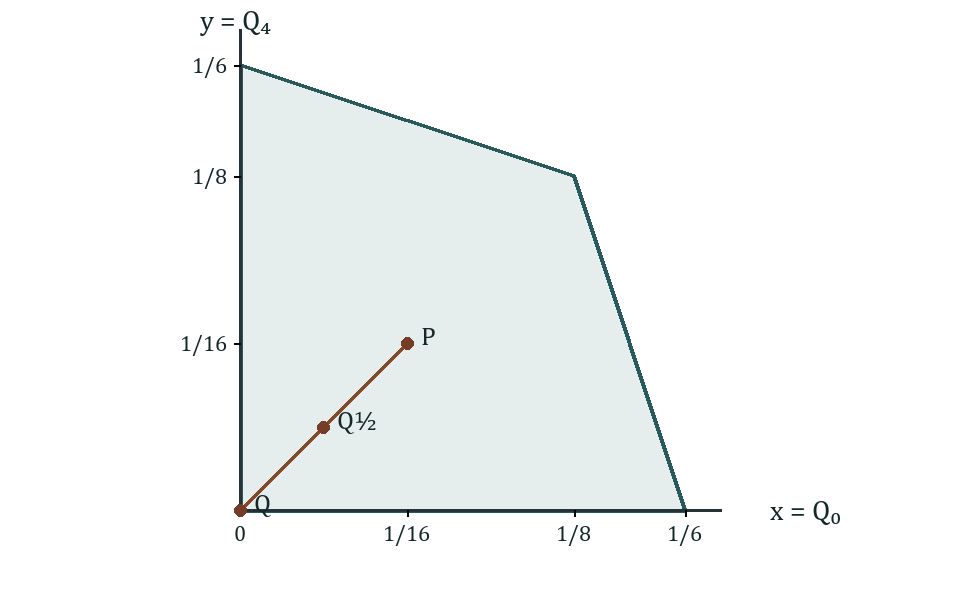
\includegraphics[width=0.63\linewidth,height=\textheight,keepaspectratio,alt={The limiting margin polytope for four-point blocks. The segment joins the boundary profile to the reference law; its midpoint is the equal mixture.}]{figures/profile_slice.png}
\par\smallskip\small\textbf{Figure 1.} The limiting margin polytope for four-point blocks. The segment joins the boundary profile to the reference law; its midpoint is the equal mixture.
\end{minipage}\end{center}

The rate also controls fluctuations directly. With natural logarithms, Pinsker's inequality gives \(D(Q\|P)\ge\|Q-P\|_1^2/2\). Indeed, group the coordinates with \(Q_j>P_j\) into one event. By the log-sum inequality the divergence dominates the binary divergence for that event. As a function of its first probability \(u\), the binary divergence has second derivative \(1/[u(1-u)]\ge4\) and vanishes to first order at the reference probability. Their difference is \(\|Q-P\|_1/2\). Applying the closed-set bound to \(\|Q-P\|_1\ge\varepsilon\) now gives, for fixed \(\varepsilon>0\), along admissible orders, \[\limsup_{n\to\infty} b_n^{-1}\log\Pr(\|Q_n-P\|_1\ge\varepsilon)
 \le -\varepsilon^2/2 .\]

\subsection{11. Formalization}\label{formalization}

The accompanying formal development proves the enumeration theorem for exact integer quotas, its upper bound allowing absent types, and the probability statement of Corollary 10.1. The formal companion identifies their declarations and follows the intermediate arguments from the incidence inverse to the rounding of profiles. Its source archive fixes Lean and the dependency revisions used in verification.

The graph omniabsorption theorem in Section 6 is imported through the Lean development of refined absorption. The companion gives the precise import and the hypotheses supplied by the construction.

\subsection{Acknowledgments}\label{acknowledgments}

The author is deeply grateful to his wife María Paz and his children Lucas, Juan Cristóbal, Francisca, Raimundo and Benjamín for their love, patience and support.

\subsection{Use of artificial intelligence and computational tools}\label{use-of-artificial-intelligence-and-computational-tools}

Claude, by Anthropic, and ChatGPT/Codex, by OpenAI, were used to explore and check arguments and to prepare the manuscript.

Certo {[}5{]} was used to explore finite instances, check identities and assess candidate constructions. These computations informed the development of the arguments; finite checks were not treated as proofs of universal statements.

The author remains responsible for the arguments, citations, code and presentation. No AI system is listed as an author.

\subsection{References}\label{references}
\raggedright

{[}1{]} P. Keevash. \emph{Counting designs}. J. Eur. Math. Soc. 20(4) (2018), 903--927, \href{https://doi.org/10.4171/JEMS/779}{doi:10.4171/JEMS/779}.

{[}2{]} J. P. Traverso Gianini. \emph{Counting Steiner triple systems and Latin squares with prescribed color statistics}. Paper II of this series, 2026. \url{https://github.com/jtraverso/color-statistics-steiner-latin}.

{[}3{]} M. Delcourt and L. Postle. \emph{Refined absorption: A new proof of the existence conjecture}. \href{https://arxiv.org/abs/2402.17855}{arXiv:2402.17855}.

{[}4{]} N. Linial and Z. Luria. \emph{An upper bound on the number of Steiner triple systems}. Random Structures Algorithms 43(4) (2013), 399--406, \href{https://doi.org/10.1002/rsa.20487}{doi:10.1002/rsa.20487}.

{[}5{]} J. P. Traverso Gianini. \emph{Certo}. Software, \url{https://github.com/jtraverso/certo-math}.

{[}6{]} J. P. Traverso Gianini. \emph{Entropy and large deviations for Latin squares}. Paper I of this series, 2026. \url{https://github.com/jtraverso/latinon-entropy-ldp/releases/tag/latinon-v1.0}.

{[}7{]} P. Keevash. \emph{Coloured and directed designs}. Building Bridges II, Bolyai Soc. Math. Stud. 28, Springer, 2019, 279--315, \href{https://doi.org/10.1007/978-3-662-59204-5_9}{doi:10.1007/978-3-662-59204-5\_9}. \href{https://arxiv.org/abs/1807.05770}{arXiv:1807.05770}.

{[}8{]} P. Keevash. \emph{The existence of designs II}. \href{https://arxiv.org/abs/1802.05900}{arXiv:1802.05900}.

{[}9{]} M. Kwan, A. Sah and M. Sawhney. \emph{Enumerating matroids and linear spaces}. Comptes Rendus. Mathématique \textbf{361} (2023), 565--575. \href{https://doi.org/10.5802/crmath.423}{doi:10.5802/crmath.423}.

{[}10{]} P. Bennett and T. Bohman. \emph{A natural barrier in random greedy hypergraph matching}. \href{https://arxiv.org/abs/1210.3581}{arXiv:1210.3581}.

\end{document}
